\documentclass[journal]{IEEEtran}

\usepackage{cite}
\usepackage{amsmath,amssymb}
\usepackage{graphicx}
\usepackage{booktabs}
\usepackage{url}

\begin{document}

\title{Memory-Aware Feature Design Dominates Quantum-Inspired\\
Architecture in Physics-Informed Solvers for\\
Time-Fractional Integro-Differential Equations}

\author{Author~Name~Placeholder%
\thanks{Department / Lab Placeholder, Institution Placeholder, City, Country
(e-mail: email@placeholder.edu).}}

\maketitle

\begin{abstract}
Physics-informed neural networks (PINNs) for time-fractional integro-differential
equations must approximate a nonlocal Caputo derivative and a weakly singular
Volterra memory term, and their accuracy is sensitive both to the numerical
treatment of those operators and to the representation given to the network. We
benchmark a classical PINN, a trainable-embedding quantum-inspired (TE) surrogate,
and analytic memory-aware input features on a manufactured fractional
integro-differential problem, under a fairness-controlled protocol with matched
parameter budgets, matched collocation points, and ten seeds per variant. A
classical-plus-memory control isolates feature-level gains from architecture-level
gains. Analytic memory features are the dominant effect: they reduce final relative
$L_2$ error by $8.66\times$ over the classical baseline ($10/10$ seeds,
$p=0.0020$). The TE surrogate also helps independently of features
($1.96\times$ over the classical baseline, $10/10$, $p=0.0020$), and the combined
TE-plus-memory model is the strongest variant overall
($0.00262\pm0.00081$). Its margin over the classical-plus-memory control is
$1.58\times$ ($9/10$, $p=0.0488$) at the primary operating point, which does not
clear a Bonferroni threshold for five comparisons, and $1.64\times$ ($9/10$,
$p=0.0098$) at an altered fractional setting $(\alpha,\beta)=(0.7,0.3)$. A
post-quantum LayerNorm variant is indistinguishable from the plain TE surrogate
($p=0.4922$). We report a zero-predictor reference ($u\equiv0$, relative
$L_2=1$) alongside every table, and we make no claim of quantum advantage: the TE
model is a classical surrogate whose sinusoidal feature map has learned,
input-dependent frequencies.
\end{abstract}

\begin{IEEEkeywords}
Physics-informed neural networks, fractional integro-differential equations,
Caputo derivative, product integration, graded meshes, quantum-inspired neural
networks, memory-aware features.
\end{IEEEkeywords}

\section{Introduction}
\IEEEPARstart{T}{ime-fractional} integro-differential systems are a demanding test
for neural solvers. Their operators are nonlocal in time, so the state at $t$
depends on accumulated history rather than on local derivatives alone, and the
kernels involved are weakly singular. Automatic differentiation cannot express a
Caputo derivative directly, so PINNs for such problems must embed a numerical
history operator inside the residual \cite{PINNs,FracPINN}.

Two directions have been proposed for improving on a baseline PINN in this
setting: architecture-level changes, of which trainable-embedding quantum
physics-informed neural networks (TE-QPINNs) are a recent instance
\cite{QNN,TEQPINN}, and feature-level priors that encode fractional-memory
structure directly in the network input. These are frequently conflated. A
quantum-inspired architecture evaluated against a plain baseline can appear to
succeed when the gain in fact comes from an accompanying change of input
representation.

This letter separates the two. We evaluate four variants against a classical
baseline under one residual construction, matched parameter counts, matched
collocation budgets, and ten seeds, and we add a \emph{classical-plus-memory}
control whose only difference from the baseline is the input representation. This
control is what makes the attribution possible, and it is absent from most
quantum-inspired PINN comparisons.

Our contributions are: (i) a fairness-controlled benchmark that separates
feature-level from architecture-level gains on a fractional integro-differential
problem; (ii) evidence that analytic memory features are the dominant effect,
larger than any architectural change we tested; (iii) evidence that the TE
surrogate contributes an independent and smaller gain, with the combined model
strongest overall; and (iv) a negative result for post-quantum LayerNorm
stabilization. We report all comparisons against an explicit zero-predictor
reference, which we argue should be standard practice in this literature.

\section{Problem and Residual Construction}

\subsection{Governing Equation}
We solve the time-fractional integro-differential equation
\begin{equation}
\begin{split}
D_t^{\alpha}u(x,t)&-(x^{2}+1)u_{xx}(x,t)\\
&+\int_{0}^{t}\sin(x)(t-s)^{-\beta}u(x,s)\,ds=f(x,t)
\end{split}
\label{eq:pde}
\end{equation}
on $x\in[0,1]$, $t\in(0,1]$, with $u(0,t)=t^{\alpha}$, $u(1,t)=-t^{\alpha}$ and
$u(x,0)=0$. Here $D_t^{\alpha}$ is the Caputo derivative
\begin{equation}
D_t^{\alpha}u(x,t)=\frac{1}{\Gamma(1-\alpha)}\int_{0}^{t}(t-s)^{-\alpha}
\partial_s u(x,s)\,ds ,
\end{equation}
and the Volterra kernel $(t-s)^{-\beta}$ is weakly singular but integrable for
$0<\beta<1$. The manufactured solution is $u_{\mathrm{exact}}(x,t)=
t^{\alpha}\cos(\pi x)$, with $f$ derived analytically under the full operator, so
that final $L_2$ and $L_\infty$ errors are computable exactly and identically
across variants.

\subsection{Discretization}
The Caputo term uses an L1 approximation on a graded temporal mesh
$t_n=T(n/N)^{r}$ with $r\ge1$ \cite{L1Scheme,GradedMesh}, which concentrates nodes
near $t=0$ where the solution's temporal derivative is singular. The Volterra term
uses kernel-aware product integration: on each interval $[t_j,t_{j+1}]$ the
solution is interpolated linearly while the singular kernel moments
$\int\tau^{-\beta}d\tau$ and $\int\tau^{1-\beta}d\tau$ are integrated analytically
\cite{ProductIntegration,VolterraCollocation}, giving
\begin{equation}
\mathcal{I}_n[u](x)\approx\sum_{j=0}^{n}w_{n,j}\,\hat u(x,t_j),
\label{eq:prodint}
\end{equation}
with weights $w_{n,j}$ depending only on the mesh and $\beta$. Verified against
the exact Beta-function value for $u=s^{\alpha}$, this rule converges at second
order (error $1.19\times10^{-4}\!\to\!1.91\times10^{-6}$ for
$N_t=25\!\to\!200$), whereas applying Gauss--Legendre quadrature to the singular
integrand stagnates near $1.7\times10^{-2}$ regardless of refinement.

Both the L1 stencil and \eqref{eq:prodint} are linear in the history values
$u(x,t_j)$. Each is therefore a fixed weight matrix applied to one history
tensor, which we assemble with a single batched network evaluation rather than one
evaluation per history node. This is algebraically exact --- residuals and
parameter gradients agree with the naive loop to $1.8\times10^{-15}$ and
$1.8\times10^{-14}$ respectively --- and reduces residual cost by about $60\times$
per step, which is what makes a ten-seed protocol at a converged budget practical.

The network minimizes
$\mathcal{L}=\lambda_{\mathrm{pde}}\mathcal{L}_{\mathrm{pde}}+
\lambda_{\mathrm{bc}}\mathcal{L}_{\mathrm{bc}}+
\lambda_{\mathrm{ic}}\mathcal{L}_{\mathrm{ic}}$ with fixed weights across all
variants.

\section{Model Variants}

\subsection{TE-Inspired Surrogate}
The TE surrogate is a classical PyTorch model that emulates TE-QPINN design ideas
\cite{TEQPINN} without a quantum circuit. Inputs are affine-rescaled; a trainable
embedding network produces $\phi_i$, from which angle-style coordinates
$\theta_i=\phi_i(x,t)\,\tilde z_i$ are formed against cycled input coordinates. The
feature map is $[\sin\theta,\cos\theta]$ augmented with pairwise terms
$\sin(\theta_i)\cos(\theta_{i+1})$, followed by a mixing block and an
expectation-style readout with an optional residual branch.

We state plainly what this is: a multilayer perceptron on a sinusoidal feature map
whose frequencies are learned and input-dependent, i.e.\ a learned Fourier-feature
model \cite{FourierFeatures}. The pairwise terms are products of independently
computed scalars and therefore factorize; they are degree-two interaction features,
not entanglement. No quantum hardware or simulator is used in the results below,
and no quantum advantage is claimed.

\subsection{Analytic Memory Features}
The memory-aware variants replace the input $(x,t)$ with
\begin{equation}
\phi_{\mathrm{mem}}(x,t)=\bigl[x,\;t,\;t^{\alpha},\;t^{1-\alpha},\;t^{1-\beta},\;
\log(1+t),\;xt,\;xt^{\alpha}\bigr],
\end{equation}
evaluated at $t_{\mathrm{safe}}=\max(t,\epsilon)$ with $\epsilon=10^{-8}$ and
normalized by deterministic, analytically derived per-feature bounds rather than
batch statistics, so train and evaluation behavior coincide. The powers
$t^{\alpha}$, $t^{1-\alpha}$, $t^{1-\beta}$ are motivated by the regularity theory
for time-fractional problems, which predicts $t^{\alpha}$-type behavior near the
origin \cite{GradedMesh}. The same feature builder is shared by the classical and
TE tracks, so no implementation asymmetry is introduced.

\section{Experimental Protocol}
All variants share \eqref{eq:pde}, the residual construction, the collocation and
boundary sampling, and the loss weights; only representation and architecture
change. The core setting is a $50\times50$ discretization with mesh grading
$r=2$, $\alpha=\beta=0.5$, and parameter counts matched within $11\%$
($2241$--$2498$). Every variant is trained for $8000$ Adam epochs with cosine
warmup, and each is run on the same ten seeds
$\{0,1,2,3,4,42,123,999,2024,2025\}$. Errors are evaluated on a uniform
$100\times100$ grid independent of the graded training mesh, and the reported
value is the error of the final model state, not the best observed during
training.

We report paired Wilcoxon signed-rank tests on final $L_2$ over the shared seeds,
bootstrap $95\%$ confidence intervals on the mean paired difference, and paired
effect sizes. With five comparisons, a Bonferroni threshold is $0.05/5=0.01$; we
state explicitly which comparisons clear it.

\emph{Zero-predictor reference.} Predicting $u\equiv0$ gives relative $L_2=1$ by
definition, and $L_\infty=\max|u_{\mathrm{exact}}|=1$ here. Any variant at or
above that line has not learned the solution, and differences among such variants
are not meaningful. We include this row in every table.

\section{Results}

\begin{table}[t]
\caption{Ten-seed results at $8000$ epochs, $\alpha=\beta=0.5$.
Runtime is single-thread CPU per run.}
\label{tab:main}
\centering
\footnotesize
\begin{tabular}{@{}lccrr@{}}
\toprule
Variant & $L_2$ (mean$\pm$std) & $L_\infty$ & Par. & s\\
\midrule
TE + memory        & $\mathbf{0.00262\pm0.00081}$ & $0.0075$ & $2498$ & $96$\\
Classical + memory & $0.00415\pm0.00173$ & $0.0107$ & $2433$ & $50$\\
TE + LayerNorm     & $0.01759\pm0.00479$ & $0.0583$ & $2338$ & $106$\\
TE fixed residual  & $0.01834\pm0.00380$ & $0.0606$ & $2306$ & $95$\\
Classical          & $0.03595\pm0.00740$ & $0.0880$ & $2241$ & $44$\\
\midrule
Zero predictor     & $1.00000$ & $1.0000$ & --- & ---\\
\bottomrule
\end{tabular}
\end{table}

\begin{table}[t]
\caption{Paired tests on final $L_2$, ten shared seeds. Bonferroni threshold for
five comparisons is $0.01$.}
\label{tab:paired}
\centering
\small
\begin{tabular}{@{}lcccc@{}}
\toprule
Comparison (A vs B) & Ratio & Wins & $p$ & $d$\\
\midrule
Classical+mem vs Classical & $8.66\times$ & $10/10$ & $0.0020$ & $-4.44$\\
TE+mem vs TE fixed         & $6.99\times$ & $10/10$ & $0.0020$ & $-4.41$\\
TE fixed vs Classical      & $1.96\times$ & $10/10$ & $0.0020$ & $-1.87$\\
TE+mem vs Classical+mem    & $1.58\times$ & $9/10$  & $0.0488$ & $-0.80$\\
TE+LayerNorm vs TE fixed   & $1.04\times$ & $7/10$  & $0.4922$ & $-0.18$\\
\bottomrule
\end{tabular}
\end{table}

\begin{figure}[t]
\centering
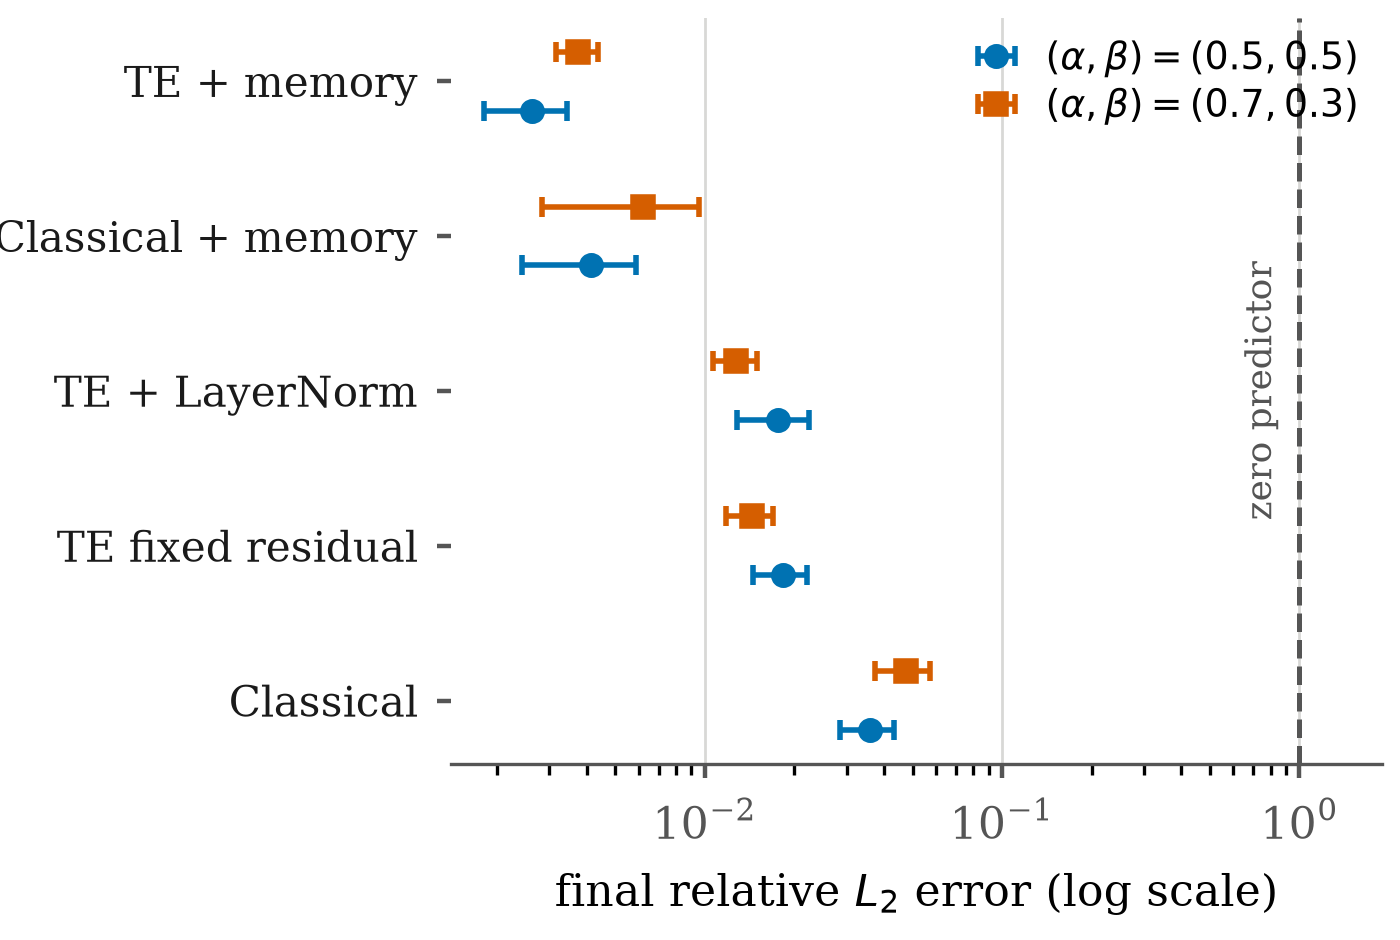
\includegraphics[width=\columnwidth]{figures/fig_results_8000ep.png}
\caption{Final relative $L_2$ error (mean $\pm$ std over ten seeds) at both
fractional settings. Memory features move a variant roughly an order of magnitude;
the TE architecture contributes a smaller additional gain. The ordering is
preserved at $(\alpha,\beta)=(0.7,0.3)$.}
\label{fig:results}
\end{figure}

\subsection{Feature-Level Versus Architecture-Level Gains}
Table~\ref{tab:main} gives the primary result and Table~\ref{tab:paired} the
paired comparisons. The largest single effect is the input representation:
classical-plus-memory improves on the classical baseline by $8.66\times$ on every
seed, with $p=0.0020$ and $d=-4.44$. The same feature set produces a comparable
$6.99\times$ improvement on the TE track. Both clear the Bonferroni threshold
comfortably.

The TE architecture also contributes independently of features: with identical
$(x,t)$ inputs, the TE surrogate improves on the classical baseline by
$1.96\times$ on every seed ($p=0.0020$). This is a genuine architectural effect,
but it is roughly a quarter the size of the feature effect.

The combined TE-plus-memory model is strongest overall. Its margin over the
classical-plus-memory control is $1.58\times$, winning $9/10$ seeds with
$p=0.0488$. We do not treat this as established: it does not clear the Bonferroni
threshold of $0.01$, and the bootstrap interval
$[-0.00266,-0.00041]$, while excluding zero, is narrow relative to the effect. It
is also the more expensive model, at roughly twice the per-epoch cost of
classical-plus-memory. We therefore report it as the leading variant rather than
as a demonstrated win.

\subsection{Stabilization}
Post-quantum LayerNorm is not supported. Against the plain TE surrogate it gives
$1.04\times$, wins $7/10$, and $p=0.4922$, with a bootstrap interval spanning
zero. At a converged budget it is indistinguishable from the variant it was
intended to stabilize.

\subsection{Robustness}
Repeating the full ten-seed protocol at $(\alpha,\beta)=(0.7,0.3)$ preserves the
ordering (Fig.~\ref{fig:results}): TE+memory $0.00375\pm0.00061$,
classical+memory $0.00617\pm0.00335$, TE+LayerNorm $0.01277\pm0.00215$, TE fixed
$0.01439\pm0.00258$, classical $0.04731\pm0.00985$. Memory features again dominate
($7.67\times$, $10/10$, $p=0.0020$) and the TE architecture again contributes
independently ($3.29\times$, $10/10$, $p=0.0020$). Notably the TE+memory margin
over classical+memory is stronger here than at the primary setting
($1.64\times$, $9/10$, $p=0.0098$), clearing the threshold that it missed above.

\subsection{Sensitivity to Training Budget}
The conclusions above depend on training to convergence, and we note this because
it changes them. Under a severely truncated budget of $12$ epochs all five
variants score at or above the zero-predictor line (final $L_2$ between $0.75$ and
$0.96$; four of five with $L_\infty>1$), and the ordering inverts: the TE
surrogate appears \emph{worst} of the group rather than second. Rankings obtained
in that regime measure initialization noise. This is a concrete argument for
reporting the zero-predictor reference: it makes such a regime immediately visible.

\section{Limitations}
The memory feature set contains $t^{\alpha}$, which is exactly the temporal factor
of the manufactured solution. A linear least-squares fit on the eight features
alone reaches relative $L_2=0.124$, against $0.362$ for $(x,t)$, so roughly a
factor of $2.9$ of the measured advantage is available before any network is
trained. The trained advantage is $8.66\times$ and therefore not explained by this
alone, but the benchmark is favorable to the feature set, and the effect should be
expected to shrink on problems whose time dependence is not $t^{\alpha}$. We
regard including $t^{\alpha}$ as principled --- $\alpha$ is a known coefficient of
\eqref{eq:pde} and the regularity theory predicts this behavior --- but the
caveat belongs with the number.

Results are for one problem family, one spatial discretization, and two
$(\alpha,\beta)$ settings. Ten seeds bound the achievable Wilcoxon $p$ from below
at $0.002$, which is adequate for the large effects but marginal for the
TE-versus-classical-memory comparison. All comparisons are equal-epoch; on an
equal-runtime basis the TE variants are penalized by roughly a factor of two.

\section{Conclusion}
Under a fairness-controlled ten-seed protocol at a converged budget, analytic
memory-aware input features are the dominant source of accuracy improvement for
PINNs on a time-fractional integro-differential problem, exceeding any
architectural change we tested by roughly a factor of four. A quantum-inspired
trainable-embedding surrogate contributes a smaller but real and independent gain,
and the combined model is strongest overall, though its margin over the
classical-plus-memory control is not established at the primary operating point.
Post-quantum LayerNorm stabilization is not supported. We recommend that
comparisons of this kind carry both a representation-matched control and an
explicit zero-predictor reference; without the first, feature-engineering gains are
readily misattributed to architecture, and without the second, rankings can be
reported from a regime in which no model has learned the solution.

\bibliographystyle{IEEEtran}
\bibliography{references}

\end{document}
